\documentclass[11pt,letterpaper]{article}

% Load some basic packages that are useful to have
% and that should be part of any LaTeX installation.
%
% be able to include figures
\usepackage{graphicx}
% get nice colors
\usepackage{xcolor}

% change default font to Palatino (looks nicer!)
\usepackage[latin1]{inputenc}
\usepackage{mathpazo}
\usepackage[T1]{fontenc}
% load some useful math symbols/fonts
\usepackage{latexsym,amsfonts,amsmath,amssymb}

% comfort package to easily set margins
\usepackage[top=1in, bottom=1in, left=1in, right=1in]{geometry}

% control some spacings
%
% spacing after a paragraph
\setlength{\parskip}{.15cm}
% indentation at the top of a new paragraph
\setlength{\parindent}{0.0cm}


\begin{document}

\begin{center}
\Large
Ay190 -- Worksheet 12\\
John Pharo\\
Date: \today\\
Starship Rangers: Mee Chatarin Wongurailertkun, David Vartanyan, Cutter Coryell
\end{center}

\section*{Problem 1}

I wrote a basic python script to read in and plot the different columns in the data file. The first column is obviously just an index; the second ranges from about 0 to $10^{34}$, which, assuming reasonable astronomical units, can only make sense as the enclosed mass. \\

The third column increases monotonically, and if we assum radius is measured in cm, then this goes to ~500 solar radii. Considering this is data from a pre-supernova massive star, that would be a reasonable measure for the total radius, so this column is probably the star's radius. \\

The next two columns decrease with radius, meaning they are probably temperature and density. However, the fifth column is monotonically decreasing, whereas the fourth fluctuates. The fourth then can't be density, because if points of higher density existed at larger radii than points of smaller density, the denser sections would just sink. Consequently, the fourth must be temperature, and the fifth density. \\

The sixth column has an interesting profile. It starts at 0, decreases sharply, then increases sharply and flatlines at zero (wrt radius). Consider than prior to a supernova, the star's core contracts sharply, faster than the local speed of sound. As a result, when the core shrinks rapidly, that information hasn't caught up to the outer atmosphere, which has yet to adjust to the new state of the star. Thus, if you consider a plot of radial velocity versus radius at this moment, the core of the star should be moving rapidly, while the atmosphere remains still. This is consistent with the plot of the sixth column. \\

The seventh column in hard to describe, so I'll just show you in Figure 1. \\

\begin{figure}[bth]
\centering
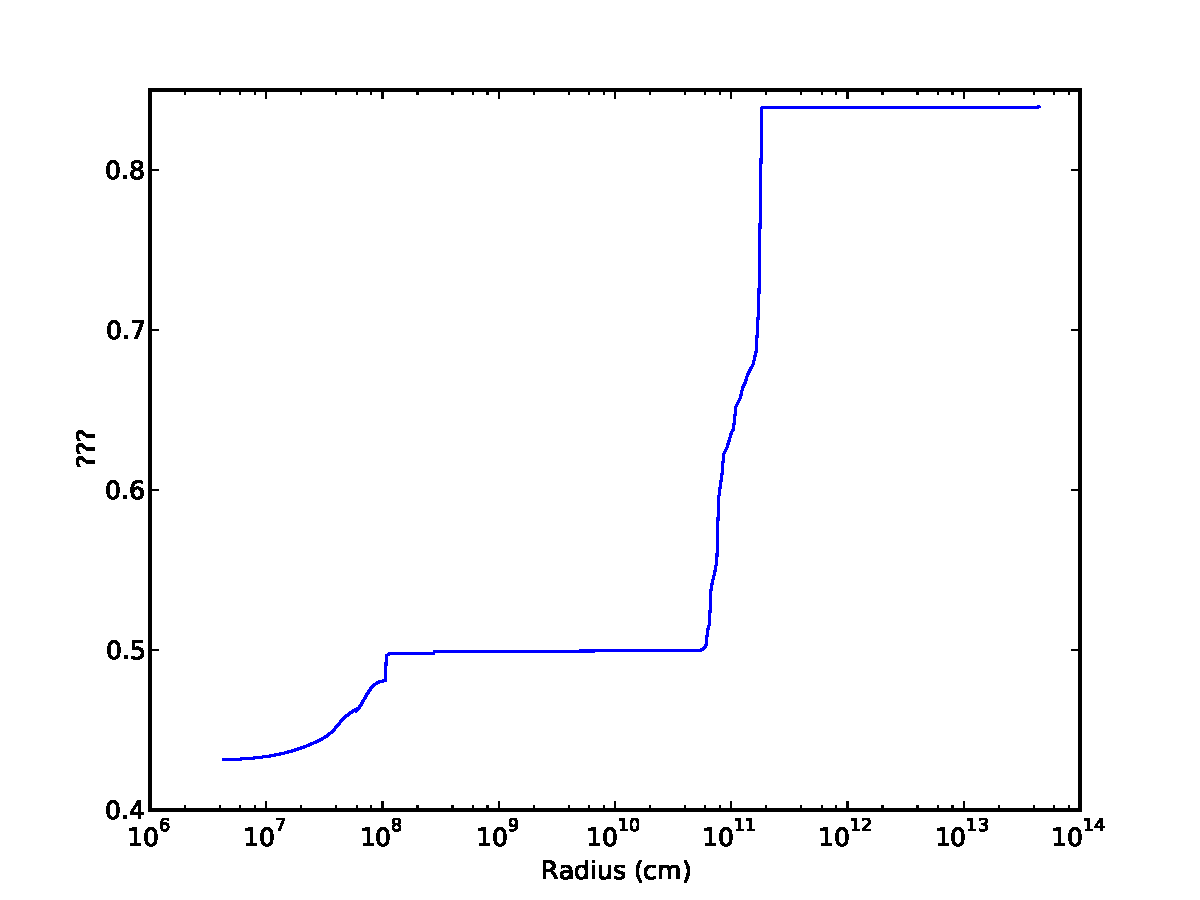
\includegraphics[width=0.5\textwidth]{EighthColumn}
\caption{This is the plot of the eighth column versus radius.}
\label{fig:simpleplot}
\end{figure}

This is the number of electrons per baryon; it maxes out at 1, at the surface, which is virtually all hydrogen, and consequently has one electron per baryon. As you move toward the center, the average element gets heavier, and has more neutrons per nucleus, to the ratio goes down.

\begin{figure}[bth]
\centering
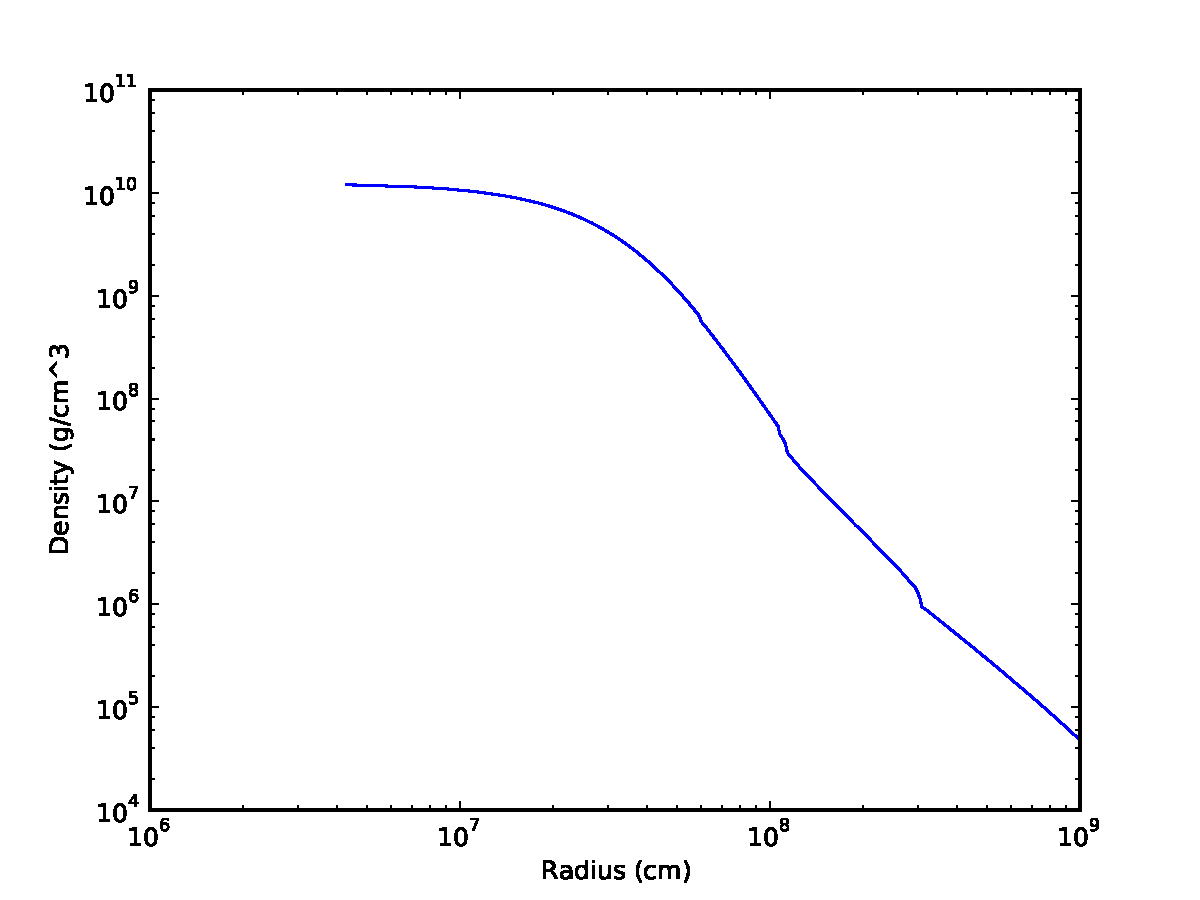
\includegraphics[width=0.5\textwidth]{Density-Radius}
\caption{This is the plot of the core density versus radius.}
\label{fig:simpleplot}
\end{figure}

\section*{Problem 2}

I use a cubic interpolation from scipy's interp1d module.

\begin{figure}[bth]
\centering
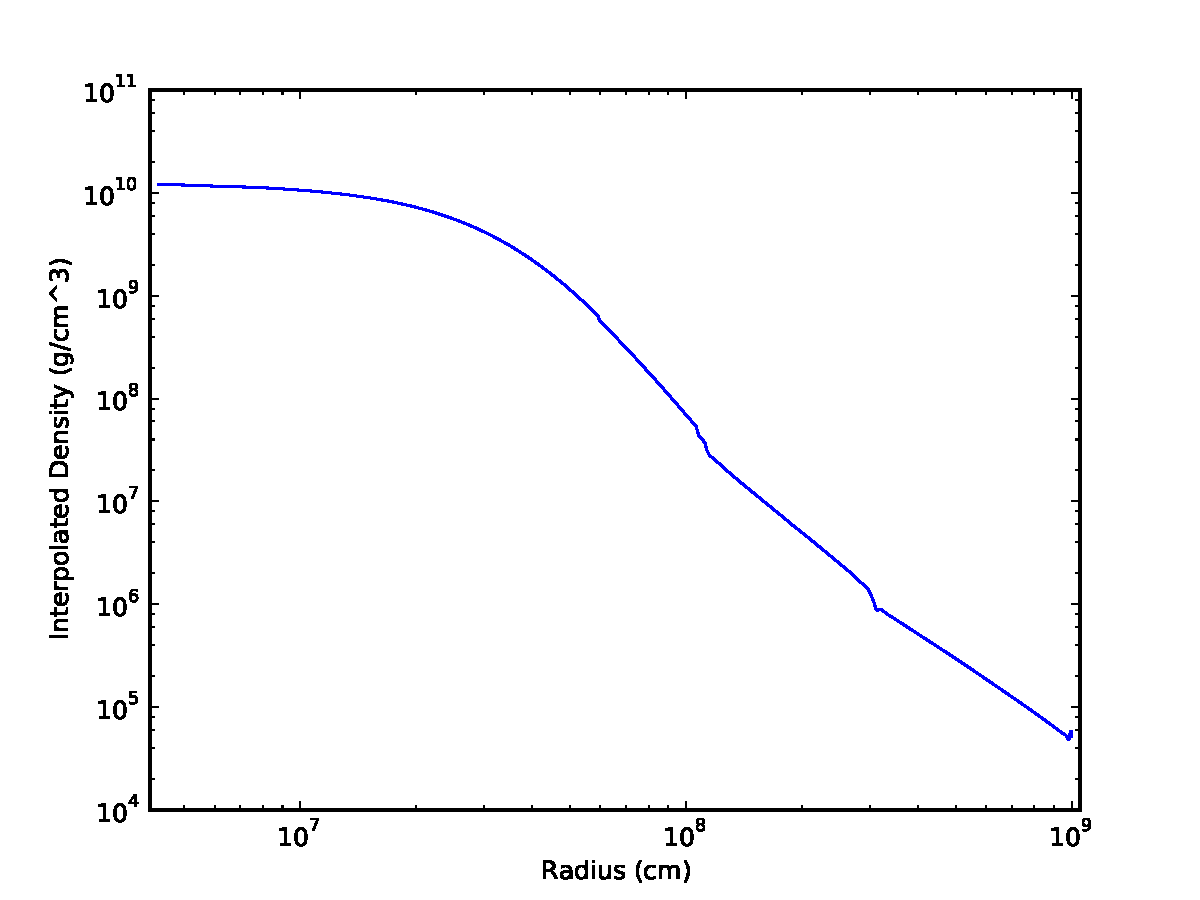
\includegraphics[width=0.5\textwidth]{Interpolation}
\caption{This is the plot of the interpolation.}
\label{fig:simpleplot}
\end{figure}

\section*{Problem 3}

See Figures 4 and 5.

\begin{figure}[bth]
\centering
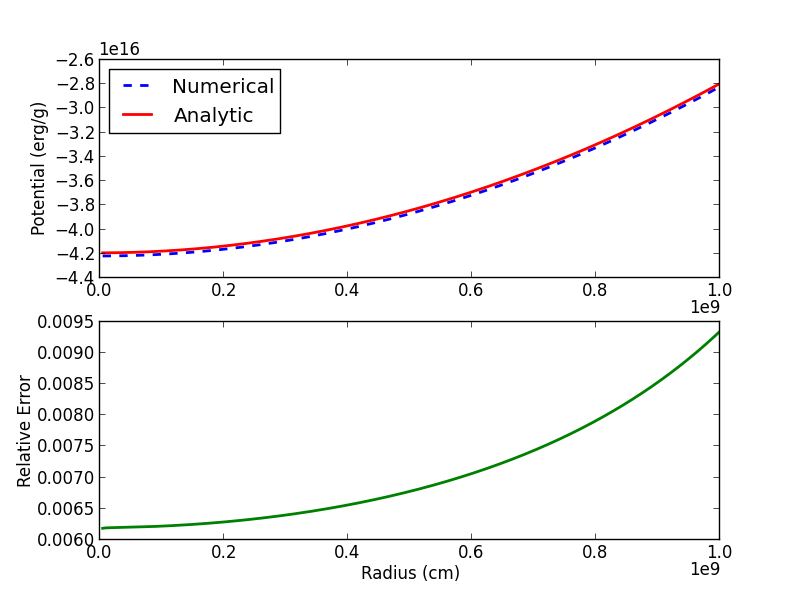
\includegraphics[width=0.5\textwidth]{Homogeneous}
\caption{This is a plot of the numerical and analytic solutions to the potential of the homogeneous sphere (with a set density of $10^5 g/cm^3$). The relative error never exceeds one percent, and the points at the surface match exactly (since the constant adjustment requires this). Calculating the convergence rate at the first points yields a rate of 1.01069547085, though the rate should be ~2. I can't figure out why this is.}
\label{fig:simpleplot}
\end{figure}

\begin{figure}[bth]
\centering
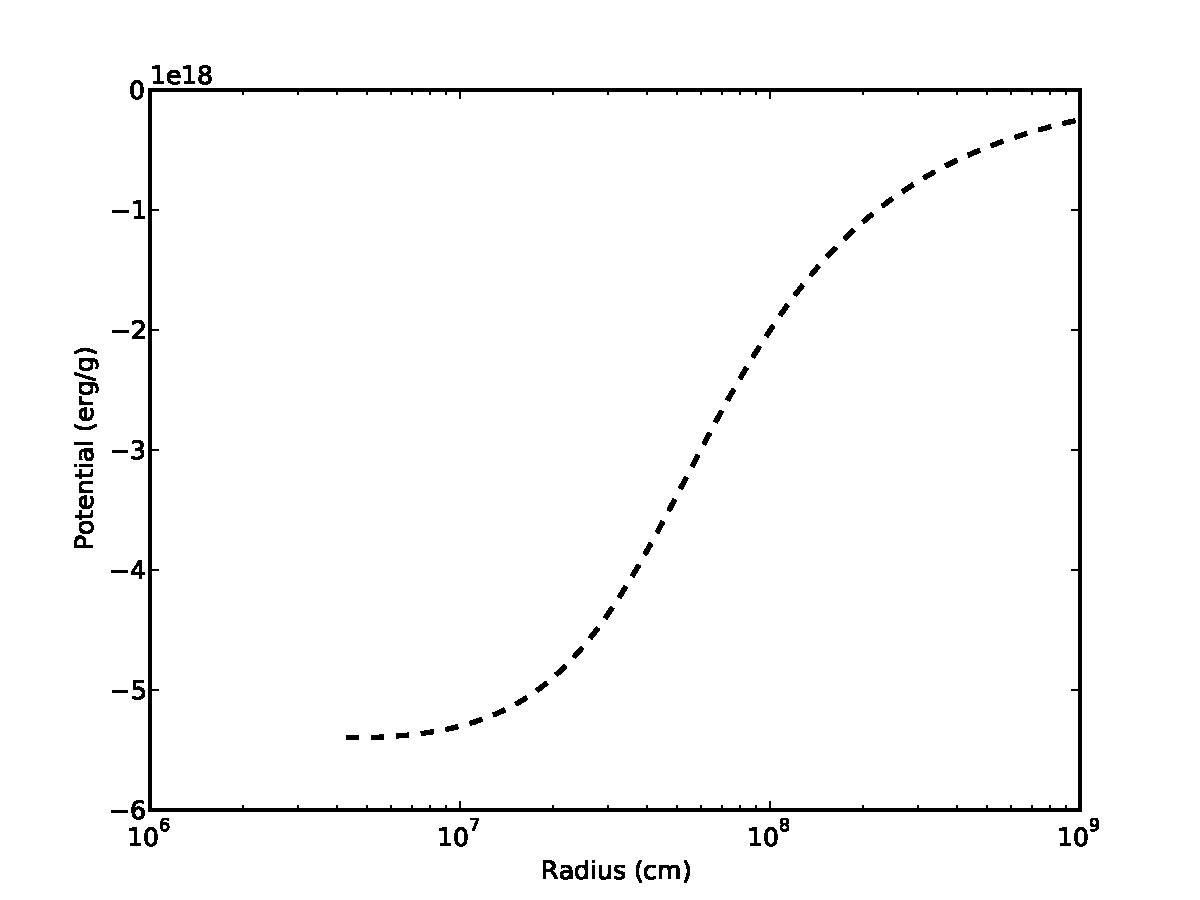
\includegraphics[width=0.5\textwidth]{Presupernova}
\caption{This is the plot of the presupernova model's potential, having validated my code for determining the potential.}
\label{fig:simpleplot}
\end{figure}

\end{document}
